% Chapter Template

\chapter{Clean Architecture} % Main chapter title

\label{Chapter5} % Change X to a consecutive number; for referencing this chapter elsewhere, use \ref{ChapterX}

\lhead{Capítulo  5. \emph{Clean Architecture}} % Change X to a consecutive number; this is for the header on each page - perhaps a shortened title

%----------------------------------------------------------------------------------------
%	SECTION 1
%----------------------------------------------------------------------------------------

\section{Modelos de Implementación Clean Architecture}

Los mejores intentos de implementación de esta arquitectura vienen de la mano de un colega Fernando Cejas y el ejemplo de los Blueprints de Google.

\begin{figure}[htbp]
	\centering
	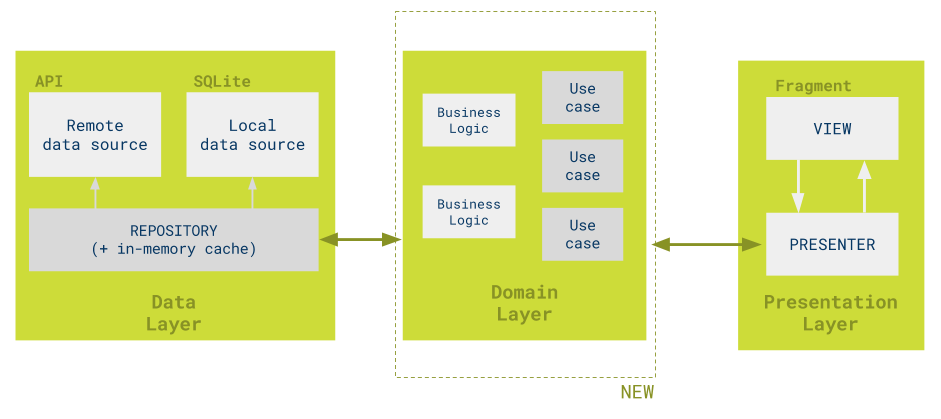
\includegraphics[width=1\textwidth]{Figures/-006.png}
	\rule{35em}{1pt}
	\caption[Principio de Dependecias]{Esquema de dependencias para una arquitectura en capas.}
	\label{fig:Diagrama_clasico}
\end{figure}

Ambas implementaciones están compuestas de tres capas distintas:

\begin{itemize}
	\item Presentation Layer: Esta capa se encarga de interactuar con la UI. Implementa un patrón de diseño conocido como \textbf{MVP (Model View Controller)}. 
	\item Domain Layer: Esta capa contiene toda la lógica de negocio. La capa de dominio comienza con las clases denominadas casos de uso o interactores según la literatura, utilizados por los presentadores de la aplicación. Estos casos de uso representan todas las acciones posibles que un desarrollador puede realizar desde la capa de presentación. Los casos de uso se implementaron utilizando el patrón de diseño conocido como \textbf{Commander}.
	\item Data Layer: Esta capa administra la adquisición de datos y es capaz de utilizar diferentes fuentes de datos. Esta capa se suele implementar utilizando el patrón de diseño conocido como \textbf{Repository}.  
\end{itemize}

\section{Presentation Layer: MVP}
El patrón de arquitectura que se utiliza en la capa de presentación de ambas implementaciones se conoce como Modelo-Vista-Presentador.
La idea detrás del patrón es concentrar la lógica de la interacción con el usuario en una entidad conocida como presentador, las operaciones directamente relacionadas con la manipulación de objetos gráficos y la captura de acciones de usuario están delegadas a la entidad Vista, finalmente la adquisición de datos y la ejecución de los algoritmos que encapsulan la lógica de negocio forman parte de las entidades modelo en el patrón.
El diagrama de componentes que describe la relación entre las partes principales se puede observar a continuación

\begin{figure}[htbp]
	\centering
	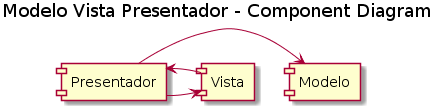
\includegraphics[width=0.7\textwidth]{Figures/uml_mvp_component.png}
	\rule{35em}{1pt}
	\caption[MVP Components]{Diagrama de componentes del patrón.}
	\label{fig:uml_mvp_component}
\end{figure}

Es posible deducir el esquema de comunicación entre los componentes a partir del diagrama. La vista se comunica de manera bidireccional con el presentador y cuando es necesario el presentador se comunica de manera unidireccional con el modelo.

\begin{figure}[htbp]
	\centering
	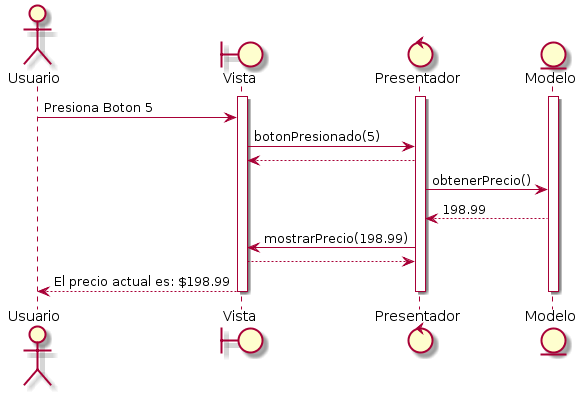
\includegraphics[width=0.7\textwidth]{Figures/uml_mvp_sequence.png}
	\rule{35em}{1pt}
	\caption[MVP Sequence]{Diagrama de secuencia para una interacción con el usuario.}
	\label{fig:uml_mvp_sequence}
\end{figure}

Una convención para la implementación del patrón es tratar de generar vistas completamente ajenas de cualquier lógica operativa y agnósticas del estado de la aplicación. Esto las convierte en un mero instrumento de interfaz entre lo que percibe el usuario y sus reacciones. 

Otra de las convenciones sugiere utilizar objetos modelo-vista en la comunicación entre el presentador y la vista para estandarizar el tipo de mensaje y el proceso de actualización de la vista.

En el caso de las implementaciones antes mencionadas la interface con el modelo es satisfecha mediante el uso de objetos casos de uso ó interactores, ambos términos siuelen utilizarse de manera intercambiable.

\section{Domain Layer: Commander Pattern}
El patrón de diseño conocido como Commander se utiliza para abstraer la ejecución de procedimientos mediante la implementación de entidades comando. Estos objetos ejecutan un único algoritmo y para ello establecen dos entidades adicionales: 
\Agregar diagrama de clases, secuencia original, secuecnia modificado por arquitectura y mapeo de entidades con entidades de arq
\begin{itemize}
	\item Solicitud (Request): Un objeto que contiene el conjunto de parametros de entrada que deben ser satisfechos para poder realizar la ejecución de la rutina del comando.
	\item Respuesta (Response): Un objeto que contiene los valores que se obtuvieron de la ejecución del algoritmo del comando.
\end{itemize}

Por lo tanto puede inferirse el flujo de operación y ejecución de los comandos.

\begin{enumerate}
\item La entidad ejecutora crea una instancia de un comando 
\item La entidad ejecutora inicializa un objeto solicitud
\item La entidad ejecutora ejecuta el comando llamando al método ''ejecutar'' de dicho comando pasando como parámetro la solicitud previamente creada.
\item La unidad ejecutora observa los resultados en espera activa implementando el patrón Observer o mediante algún esquema de callback.
\end{enumerate}

\begin{figure}[htbp]
	\centering
	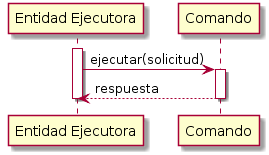
\includegraphics[width=0.5\textwidth]{Figures/uml_commander_sequence.png}
	\rule{35em}{1pt}
	\caption[MVP Components]{Diagrama de secuencia para el patrón Commander.}
	\label{fig:uml_commander_sequence}
\end{figure}

Siguiendo los lineamientos de la arquitectura propuesta los autores denominan a los comandos: Casos de Uso, ó Interactores.

Como una nota relevante de implementación se recomienda ejecutar las rutinas de los comandos en un hilo/proceso separado para para evitar bloquear el proceso principal de la apliación.

\section{Data Layer: Repository Pattern}
En la capa de datos se propone la implenentación de un patrón de diseño conocido como Repository(Repositorio). Este diseño intenta encapsular todas los orígenes de datos en una única interface. Para ello se define un objeto Repositorio que implementa la interfaz de orígen de datos. Así mismo otros objetos conocidos como Orígenes implementan la misma interfaz pero acceden distintas fuentes. La responsabilidad del Repositorio es determinar cual de esos orígen debe utilizarse para obtener los resultados para una determinada consulta de datos.
Por lo tanto la entidad que realiza la consulta de datos sólo debe conocer un sólo contrato, aquél de los Orígenes.
% 
